\section{Entanglement generation}\label{sec:4:entanglement-generation}
The averaged state $\mean{\rho}$ after multiple measurements is given by
\begin{equation}\label{eq:4:average-density}
  \mean{\rho} = \int_{-\infty}^{\infty} \dd \theta_A p(\theta_A) \int_{-\infty}^{\infty} \dd \theta_B p(\theta_B) \int_{-\infty}^{\infty} \dd L_A p(L_A) \int_{-\infty}^{\infty} \dd L_B p(L_B) \ \rho(\theta_A, \theta_B, L_A, L_B)
\end{equation} 
where $p(\,\cdot\,)$ represents the Gaussian distributions of the random variables 
$\theta_{A(B)}$ and $L_{A(B)}$ with standard deviations $\Delta \theta$ or $\Delta L$ respectively. 
$\rho(\theta_A, \theta_B, L_A, L_B)$ denotes the state of a single measurement, dependent on the initial setup of the system.
The state $\rho_0$ at $t=0$ is given as before by eq. \eqref{eq:2:initial-state}.
Additionally to mutual gravitational coupling, the Casimir interactions of the state $\ket{\psi^{(i)}_{A(B)}}$ ($i = 1, 2$) with the Faraday shield induce the dynamic phase $\phi^{(i)}_{A(B),\,\mathrm{Cas}}(t)$.
Using the two different models for the Casimir attraction for large and small separations given by eq. \eqref{eq:3:casimir-sphere-plate-PFA} and eq. \eqref{eq:3:casimir-sphere-plate-PFA}, it follows
\begin{equation}
  \phi^{(i)}_{A(B),\,\mathrm{Cas}}(t) = \frac{t}{\hbar}
  \begin{cases}
     \frac{3 \hbar c}{8 \pi} \left(\frac{\varepsilon_r - 1}{\varepsilon_r + 2}\right) \frac{R^3}{\left(L^{(i)}_{A(B)}\right)^4} & \text{for large separations (LSL)} \\
    \frac{\hbar c \pi^3}{720} \varphi(\varepsilon_r) \left(\frac{\varepsilon_r - 1}{\varepsilon_r + 1}\right) \frac{R}{\left(\mathscr{L}^{(i)}_{A(B)}\right)^2} & \text{for small separations (PFA) .}
  \end{cases}
\end{equation}
Here, $L^{(i)}_{A(B)}$ and $\mathscr{L}^{(i)}_{A(B)} = L^{(i)}_{A(B)}-R$ are the  distances between the particles and the shield's surface given by
\begin{align}\label{eq:4:L-casimir}
  L^{(i)}_{A} &= L + L_{A} - \frac{d}{2} \pm_i \frac{\Delta x_{A}}{2} \sin(\alpha + \theta_{A}) \quad \quad \text{and} \\
  L^{(i)}_{B} &= L + L_{B} - \frac{d}{2} \mp_i \frac{\Delta x_{B}}{2} \sin(\beta + \theta_{B})
\end{align}
where $\pm_i = -(-1)^{i}$ distinct between the two cat-states of a single particle.
The phase imprinted by the mutual gravitational interactions between states $\ket{\psi^{(i)}_A}\otimes\ket{\psi^{(j)}_B}$ is given analogue to the previous calculations in \cref{cha:first-look} as
\begin{equation}\label{eq:4:phi-grav}
  \phi^{(ij)}_\mathrm{Grav}(t) = \frac{t}{\hbar} \frac{G M_A M_B}{L^{(ij)}} .
\end{equation}
The separation $L^{(ij)}$ between the particle cat-states $A^{(i)}$ and $B^{(j)}$ is given by
\begin{multline}\label{eq:4:L-gravity}
  L^{(ij)} = \sqrt{\left(2L + L_A + L_B \pm_i \frac{\Delta x_A}{2}\sin(\alpha + \theta_A) \mp_j \frac{\Delta x_B}{2}\sin(\beta + \theta_B)\right)^2 +} \\ \overline{\left(\frac{\Delta x_A}{2}\cos(\alpha + \theta_A) \mp_{i=j} \frac{\Delta x_B}{2}\cos(\beta + \theta_B)\right)^2}
\end{multline}
with $\mp_{i=j} = +(-1)^{\delta_{ij}}$.
Expanding to first order in $\Delta x_{A(B)} \ll L$, $\theta_{A(B)} \ll 1$ and $L_{A(B)} \ll 1$ (which is justified as seen in the following), the averaged evolved state 
$\mean{\rho}$ in eq. \eqref{eq:4:average-density} is analytically obtainable, as shown in \cref{apx:placement-average-density-matrix}.
Assuming $\Delta \theta_A = \Delta \theta_B \equiv \Delta\theta$ and $\Delta L_A = \Delta L_B \equiv \Delta L$, the off-diagonal elements (the so-called \textit{coherences}) decay with
\begin{equation}\label{eq:4:average-density-element}
  \mean{\rho_{kl}} = \frac{1}{4} e^{i \Delta \phi_{kl}(t)} \exp{-\frac{(\xi_{kl})^2}{2} (\Delta\theta)^2 t^2} \exp{-\frac{(\zeta_{kl})^2}{2} (\Delta L)^2 t^2}
\end{equation}
where $\Delta \phi$, $\xi$ and $\zeta$ are substitutes for lengthy expressions given by eq. \eqref{eq:apx:phi-definition}, eq. \eqref{eq:apx:definition-xi} and eq. \eqref{eq:apx:definition-zeta} in the appendix and are dependent on system parameters.
For $\Delta \theta, \Delta L \rightarrow \infty$ or $t\rightarrow \infty$, coherences vanish, resulting in a maximally mixed state with $\tr\rho^2 = 1/4$ - which is not entangled.
For large variations in the initial placement of the particles, one therefore expects the loss of entanglement.

In the special case of two identical particles and $\alpha=\pm\beta$, the logarithmic negativity is approximated in first order by
\begin{equation}\label{eq:4:log-neg-analytical}
  E_N(\mean{\rho}) = \max\left\{ 0,\ \log_2\left(e^{-\gamma}\left(\cosh\gamma + \abs{\sin \phi}\right)\right) \right\}
\end{equation}
where the decoherences $\gamma = \left(\xi^2(\Delta \theta)^2/2 + \zeta^2(\Delta L)^2/2\right)t^2$ are shown in eq. \eqref{eq:apx:stochastic-decoherence} and the phase $\phi$ is given by eq. \eqref{eq:4:phi-orientation} in the next section.
Numeric results confirm the first order approximation and are shown in \cref{fig:4:EN-variations} for different values of $\Delta \theta$ and $\Delta L$ in the parallel configuration.
\begin{figure}[!htb]
  \centering
  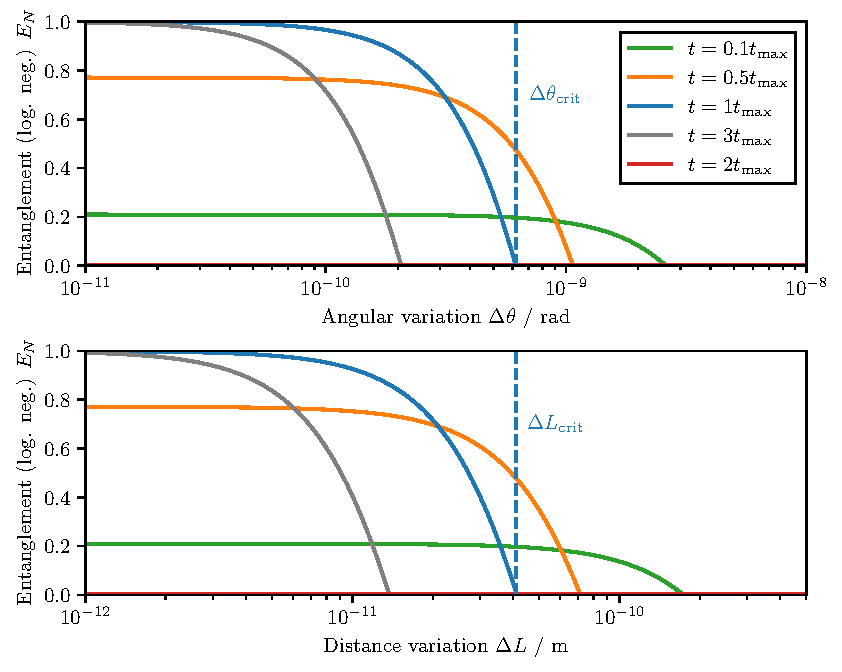
\includegraphics[width=\textwidth]{./../figures/theta-variance/EN-deltaTheta-deltaL.pdf}
  \caption{Entanglement quantified by the logarithmic negativity (eq. \eqref{eq:2:logarithmic-negativity}) dependent on the angular variation $\Delta\theta$ and the distance variation $\Delta L$ in the parallel configuration. The entanglement is shown at different times, where $t_\mathrm{max} \approx 258\si{ms}$ is the time of maximal entanglement from eq. \eqref{eq:2:t-max-parallel}. At the critical point $\Delta \theta_\mathrm{crit}$ or $\Delta L_\mathrm{crit}$ all entanglement is lost.}
  \label{fig:4:EN-variations}
\end{figure}
For small placement variations, entanglement is virtually unaffected but at the critical thresholds $\Delta \theta_\mathrm{crit}$ and $\Delta L_\mathrm{crit}$ entanglement is completely lost.
The critical decoherence $\gamma_\mathrm{crit}$ is given by
\begin{equation}\label{eq:4:critical-point}
  \gamma_\mathrm{crit} = \log(1 + \sqrt{2}) = \mathrm{const.}
\end{equation}
resulting in $\Delta\theta_\mathrm{crit} \propto 1/(\xi t)$ and $\Delta L_\mathrm{crit} \propto 1/(\zeta t)$. 
For the used parameters shown in \cref{tab:paramters}, the threshold is around $\Delta \theta_\mathrm{crit} \approx 6 \times 10^{-10} \si{rad}$ and $\Delta L_\mathrm{crit} \approx 1.4 \times 10^{-10} \si{m}$, which seems quite challenging experimentally.
\begin{table}[!t]
  \centering
  \begin{adjustbox}{max width=\textwidth}
    \begin{tabularx}{\textwidth}{c c c c c c c}
      \toprule
      \multirow{2}{*}{Orientation} & \multicolumn{2}{c}{Particle size} & \multirow{2}{*}{$L$} & \multirow{2}{*}{$\Delta x$} & \multicolumn{2}{c}{Shield size $^b$} \\ \cline{2-3} \cline{6-7}
      & Radius $R$ & Mass $M$ $^a$ & & & $d$ & $r_s$\\
      \midrule
      \begin{tabular}{@{}c@{}}Parallel \\ ($\alpha=\beta=0$) \end{tabular} & \begin{tabular}{@{}c@{}}$10\si{\mu m}$ \\ $=10^{-5}\si{m}$\end{tabular} & \begin{tabular}{@{}c@{}}$\approx 10^{-11}\si{kg}$ \\ $=5\times 10^{-4} \, m_p$\end{tabular} & $2R=20\si{\mu m}$ & $100\si{nm}$ & $100\si{nm}$ & $1\si{cm}$ \\
      \bottomrule
      \multicolumn{7}{l}{\footnotesize $^a$ Here $m_p = \sqrt{c\hbar/G}\approx 2.17\times 10^{-8}\si{kg}$ is the Planck mass. $^b$ The required size of the shield is later} \\[-4pt]
      \multicolumn{7}{l}{\footnotesize estimated in section 5.1.} \\[5pt]
    \end{tabularx}
  \end{adjustbox}
  \caption{Default parameters for the setup in \cref{fig:4:complete-setup}. Maximum entanglement is reached after $t_\mathrm{max} = 259\si{ms}$ for these parameters. They were chosen in accordance with multiple proposals \cite{Aspelmeyer_2024,Rijavec_2021}. Both particles are assumed to be identical. The thickness $d$ and radius $r_s$ of the shield is estimated in \cref{sec:5:shield-size}.}
  \label{tab:paramters}
\end{table}
For all these calculations, the radius of the particles was set to $R=10^{-5}\si{m} = 10\si{\mu m}$ with corresponding masses $M=4/3 \pi R^3 \rho_\mathrm{Silica} \approx 1.1\times 10^{-11}\si{kg}$.
A particle-shield separation of $L=2R$ and a superposition size of $\Delta x = 100\si{nm}$ were chosen. In the rest of this thesis, if not otherwise specified, these parameters are used as a default.
For convenient retrieval, they are collectively displayed in \cref{tab:paramters}.

These values agree with the parameter regime typically considered for such experiments \cite[Timestamp: 51:00]{Aspelmeyer_2024}, as they result in a low one-run duration of $t_\mathrm{max}\approx 258\si{ms}$.
Other proposals suggest a similar parameter set generally differing only by single orders of magnitude (see e.g. the Tab. 1 in Ref. \cite{Rijavec_2021}).
It is important however to note, that these parameters are far beyond current experimental capabilities:
The largest mass studied in matter-wave interferometry is about $4\times 10^{-23}\si{kg}$ \cite{Fein_2019} with a spatial superposition size of $\Delta x \gtrsim 500\si{nm}$.
In solid-state mechanical systems, quantum control and ground-state cooling have been demonstrated with masses of $10^{-13}\si{kg}$ for mechanical oscillators coupled to superconducting qubits \cite{OConnell_2010}; entangled diamonds with $10^{-11}\si{kg}$ have been observed \cite{Lee_2011} and masses of $10^{-8}\si{kg}$ have been prepared in motional center-of-mass cat-states \cite{Bild_2023}, although with very short coherence times $\lesssim 1\si{\mu s}$.
Also impressive and notable is the cooling of the $\sim 40\si{kg}$ LIGO mirrors to only very few occupied phonon states \cite{Whittle_2021}.
In contrast, the smallest mass with a measurable gravitational force is around $92 \si{mg}$ \cite{Westphal_2021}.
The field of levitated nano-particles has the potential to bridge molecular superposition and mechanical systems, offering exceptional quantum control, high force sensitivity and long coherence times up to seconds \cite{Aspelmeyer_2024}.
Thus many proposals aim to measure quantum entanglement due to gravity between trapped and levitated particles \cite{Krisnanda_2020,GonzalezBallestero_2021}.

Nonetheless, the required accuracy in the placement of the particles appears very challenging experimentally.
However, looking at the entanglement dynamics in \cref{fig:4:EN-dynamics-variations}, for shorter times $t<t_\mathrm{max}$, greater variations in particle placement can be tolerated at the cost of reduced entanglement.
\begin{figure}[!htbp]
  \centering
  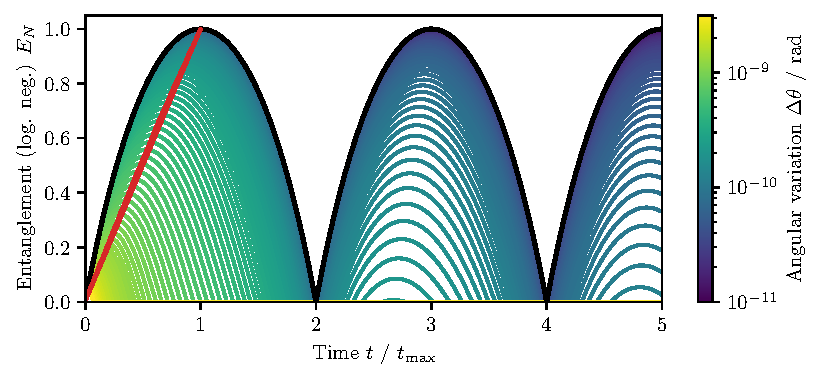
\includegraphics[width=\textwidth]{./../figures/theta-variance/EN-dynamics-delta-theta.pdf}
  \caption{Entanglement dynamics for different angular variations $\Delta \theta$ according to eq. \eqref{eq:4:log-neg-analytical}. For high variations, entanglement is only measurable for a very short amount of time. The red line shows the time, after the most amount of entanglement is measurable. The black outer most curve corresponds to the ideal scenario without any angular variations and precisely aligns with \cref{fig:2:entanglement-dynamics}.}
  \label{fig:4:EN-dynamics-variations}
\end{figure}
At these shorter times, the gravitational interaction has not fully entangled the particles, and decoherence (which scales as $\gamma \propto t^2$) has not yet significantly developed.
If achieving full entanglement is not required and \textit{any} amount of entanglement $E_N > 0$ suffices, it may be advantageous to perform measurements at $t < t_\mathrm{max}$.
This, of course, requires ensuring that other entanglement mechanisms, such as direct or indirect coupling, contribute smaller entanglement rates (see \cref{cha:the-shield} for further discussion).
Additionally, decoherence effects from collisions with air molecules and thermal black-body radiation should be taken into account.
The optimal measurement time for a required level of entanglement is depicted in \cref{fig:4:time-delta-theta}.
\begin{figure}[!htbp]
  \centering
  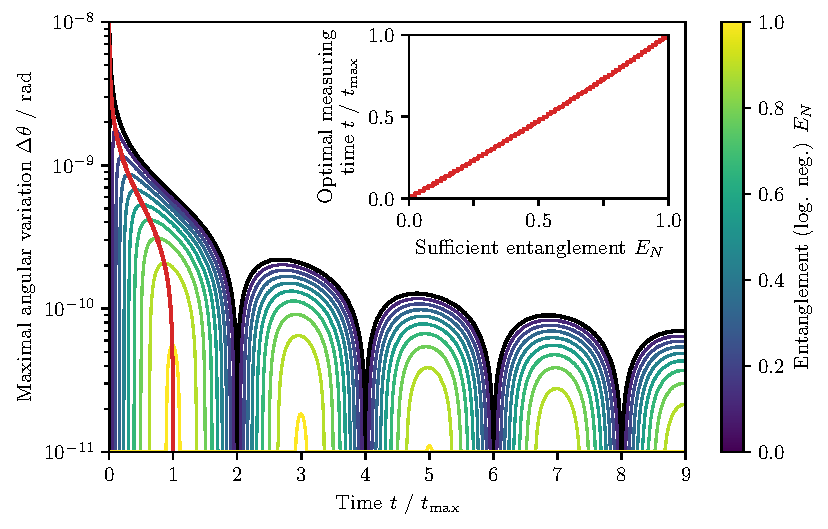
\includegraphics[width=\textwidth]{./../figures/theta-variance/time-delta-theta-crit-EN.pdf}
  \caption{Maximal angular variation for given times after which a specific amount of entanglement $E_N$ is still measurable. The setup parameters are taken from \cref{tab:paramters}. The outer most black line corresponds to the time dependence of $\Delta \theta_\mathrm{crit}$. A fully entangled state with $E_N=1$ is only measurable at $t=t_\mathrm{max}$ with a maximally possible angular variation of around $10^{-11}\si{rad}$. The red curve on the top left shows the optimal measuring time for a specific amount of entanglement and aligns precisely with the red curve in \cref{fig:4:EN-dynamics-variations}. Correspondingly, the red curve in the main figure shows the maximal angular variation for which this goal is reachable. At times $2k t_\mathrm{max},\,k\in\mathbb{N}$ no entanglement can be measured.}
  \label{fig:4:time-delta-theta}
\end{figure}
The figure also provides the corresponding maximum allowable variation for a given time. Conversely, for fixed variations, the optimal measurement time and maximum attainable entanglement can be determined.
It also can be seen that at times $2k t_\mathrm{max}, \ k\in\mathbb{N}$ no entanglement is measurable, coinciding with the findings for the ideal scenario in \cref{cha:first-look}. 
